\subsection{Dimensionality Reduction}
It takes a lot of computing power to process and interpret high-dimensional data. The data experiences the so-called \textit{curse of dimensionality}, becoming sparser as the size of the feature space expands. By projecting features onto lower-dimensional subspaces and learning from them, dimensionality reduction techniques aid in the retention of the most relevant information and improve visualisation. In this section, we experiment with several manifold and projection based learning strategies. Even while they are effective, linear dimension reduction frameworks frequently overlook significant non-linear structures in the data, which manifold learning is more sensitive to and can better generalise. We analyse the clustering outcomes of the below approaches to see which yields the best results using the original dataset with its 13 attributes as our baseline.

\subsubsection{Methods}
\textbf{PCA} - is a standard approach for linear dimensionality reduction. We fit PCA on the normalised audio features and chose the number of components that produce 95\% of the cumulative explained variance, which in our case is 7. The visualisation for this is included in Appendix \ref{appendix:B}.

\textbf{UMAP} - is a non-linear manifold learning-based method that preserves the topological structure of points in a high-dimensional space in a lower-dimensional embedding space and employs Riemannian geometry to demonstrate the connectedness of related data points as clusters. All data points are grouped based on similarities in feature values, and similar groups are positioned closer. These are the local and global structures of the map. While UMAP is a great tool for generating visualisations, we use it more generally as a data transformer \cite{umap}. While \textit{min\_dist} is the minimal distance that controls how closely or loosely the clusters will be grouped in the low dimensional space, the parameter \textit{n\_neighbors} governs the number of neighbouring data points that define the local structures of the data in the feature space. 15 nearest neighbours are considered for our scaled audio features data set at a distance of 0.1 using the default \textit{n\_components}, 2. We also perform a grid search over these hyperparameters. The choice of the results is explained in Appendix \ref{appendix:B}.

\textbf{Gaussian Random Projection} - by exchanging a controllable amount of accuracy as additional variance for quicker processing times and smaller model sizes, the \textit{random\_projection} module of the \textit{scikit-learn} library implements a straightforward and computationally effective method for reducing the dimensionality of data \cite{randomprojections}. The Johnson-Lindenstrauss lemma is the primary theoretical finding that underlies the effectiveness of random projection. The lemma infers conclusions regarding low-distortion embeddings of points from high-dimensional into low-dimensional Euclidean space such that the distances between the points are almost preserved. The Gaussian Random Projection lowers the dimensionality by mapping the initial input space onto a randomly generated matrix, whose elements are selected from the following distribution - $N(0,\frac{1}{n\_{components}})$\cite{randomprojectionssklearn}. We set \textit{n\_components} to 2.

\textbf{PaCMAP} - in contrast to earlier manifold-based dimensionality reduction algorithms that either emphasise retaining local or global trends, PaCMAP with the correct settings can represent both equally. It uses three different types of pairs of data points: neighbour pairs (\textit{pair\_neighbors}), mid-near pairs (\textit{pair\_MN}), and further pairs (\textit{pair\_FP}) \cite{pacmap}. These values determine the number of closest neighbours to take into account, the proportion of mid-near pairs to the number of neighbours, and the proportion of further pairs to the number of neighbours, respectively. The feature space is transformed using PaCMAP with its default parameter values for \textit{n\_neighbours}, 10 and number of components, 2. The scaled audio feature values are then fit into this new space.

\textbf{Autoencoders} - are a class of neural networks that learn representations from data in an unsupervised manner and are typically used for dimensionality reduction and data regeneration. They consist of two primary components, an encoder and a decoder, each of which is represented by a family of parameterised functions - the encoder family ${\displaystyle E_{\math{\phi}}:{\mathcal{X}}\rightarrow {\mathcal{Z}}}$, parameterised by ${\displaystyle\math{\phi}}$ and the decoder family ${\displaystyle D_{\math{\theta}}:{\mathcal {Z}}\rightarrow {\mathcal {X}}}$, parameterised by ${\displaystyle \math{\theta}}$. The encoder maps features from a high dimensional data space ${\displaystyle\mathcal{X}}$ to a low dimensional latent space ${\displaystyle\mathcal{Z}}$ \cite{autoencoders}. The feed-forward architecture of our symmetrical autoencoder model is made of up two layers. A fully linked dense layer, a batch normalisation layer, and the Leaky ReLU activation function are all included in each portion of the encoder and decoder blocks. We restrict the bottleneck layer to 6 dimensions and train the model on the scaled audio features. The latent feature vector produced by the encoder - ${\displaystyle z=E_{\math{\phi} }(x)}$ is then used for clustering.

\subsection{Clustering}
\subsubsection{Methods}
We are able to represent the audio characteristics of the songs using the various sets of extracted features from the dimensionality reduction techniques outlined above. We compare the performance of three clustering algorithms: K-Means, DBSCAN, and BIRCH, on these new features and the original non-reduced dataset with 13 audio features. The clustering results for the various methods are included in Appendix \ref{appendix:C}.

\textbf{K-Means} - is an effective unsupervised machine learning algorithm that divides \textit{n} observations into \textit{k} clusters, each containing points that belong to the closest mean (also known as the cluster centroid and functions as the cluster's prototype). As a result, the data space gets partitioned into several Voronoi cells \cite{kmeans}. The algorithm minimises within-cluster variances (squared Euclidean distances), termed named inertia. We use the \textit{k-means++} initialisation approach provided by \textit{scikit-learn} library to position the centroids far apart from one another. Since the euclidean distance is explosive in high-dimensional spaces, we reason that K-Means will adapt and scale well and efficiently to our implementations using dimensionality reduction. We use the Elbow method with distortion scores to determine the optimal number of clusters for each feature set.

The knee of the elbow plot is where adding a new cluster does not enhance the quality of the existing ones; and rather leads to overfitting. This strategy provides us with a sufficient number of clusters to use for each of the feature extraction strategies, as seen in \ref{fig:elbowplots}, with sizes mostly varying between 8 and 13.

\begin{figure}[!hbt]
\begin{subfigure}{.5\textwidth}
  \centering
  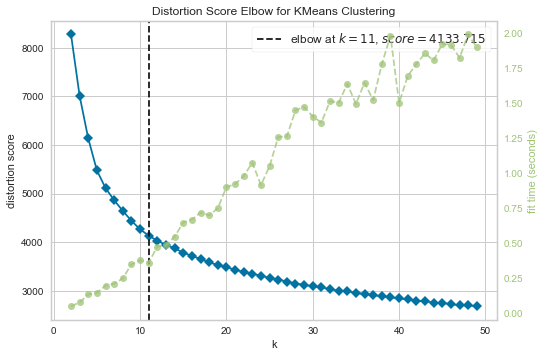
\includegraphics[width=.6\linewidth]{Outputs/Elbow Plot - Original Audio Features.png}  
  \captionsetup{justification=centering,margin=1cm}
  \caption{Number clusters for the original audio features}
  \label{fig:sub-first}
\end{subfigure}
\begin{subfigure}{.5\textwidth}
  \centering
  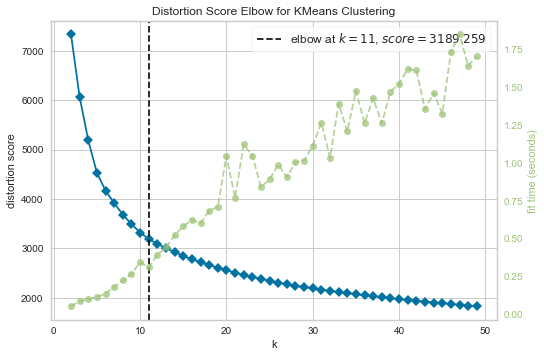
\includegraphics[width=.6\linewidth]{Outputs/Elbow Plot - PCA Features.png}  
  \captionsetup{justification=centering,margin=1cm}
  \caption{Number of clusters for the PCA audio features}
  \label{fig:sub-second}
\end{subfigure}
\medskip
\begin{subfigure}{.5\textwidth}
  \centering
  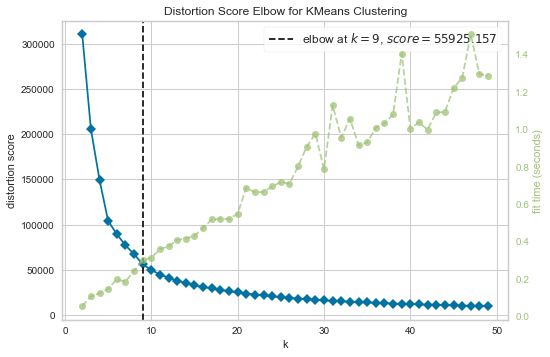
\includegraphics[width=.6\linewidth]{Outputs/Elbow Plot - UMAP Features.png}  
  \captionsetup{justification=centering,margin=1cm}
  \caption{Number of clusters for UMAP audio features}
  \label{fig:sub-third}
\end{subfigure}
\begin{subfigure}{.5\textwidth}
  \centering
  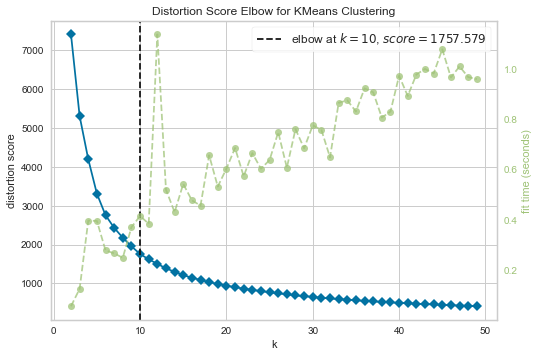
\includegraphics[width=.6\linewidth]{Outputs/Elbow Plot - Gaussian Random Projections.png} 
  \captionsetup{justification=centering,margin=1cm}
  \caption{Number of clusters for the Gaussian Random Projection audio features}
  \label{fig:sub-fourth}
\end{subfigure}
\medskip
\begin{subfigure}{.5\textwidth}
  \centering
  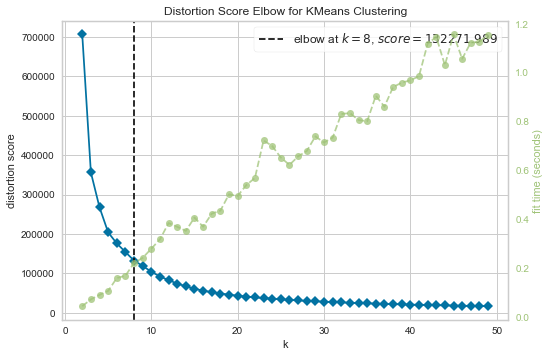
\includegraphics[width=.6\linewidth]{Outputs/Elbow Plot - PaCMAP Features.png} 
  \captionsetup{justification=centering,margin=1cm}
  \caption{Number of clusters for the PaCMAP audio features}
  \label{fig:sub-fifth}
\end{subfigure}
\begin{subfigure}{.5\textwidth}
  \centering
  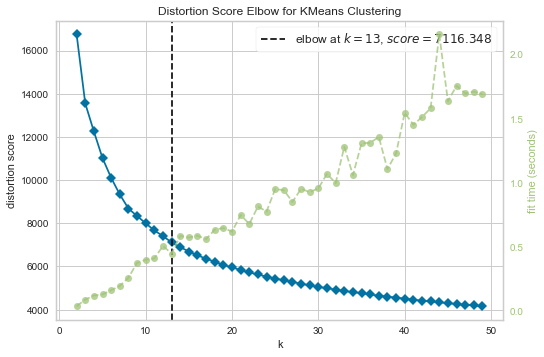
\includegraphics[width=.6\linewidth]{Outputs/Elbow Plot - Autoencoder Features.png}  
  \captionsetup{justification=centering,margin=1cm}
  \caption{Number of clusters for the Autoencoder audio features}
  \label{fig:sub-sixth}
\end{subfigure}
\caption{Elbow plots representing the optimal number of clusters with various dimensionality reduction algorithms for K-Means}
\label{fig:elbowplots}
\end{figure}
\setlength{\textfloatsep}{5pt}
\textbf{DBSCAN} - is a density-based clustering algorithm. The underlying concept is that a cluster in data space is viewed as a contiguous zone of high point density that is removed from other similar clusters by continuous regions of low point density. It can find clusters of various sizes and forms from data that contains vast amounts of noise and outliers. The two main parameters of the algorithm, \textit{min\_samples} and \textit{eps}, are what give us this notion of density. Higher \textit{min\_samples} or lower \textit{eps} imply a cluster requires a higher density to develop. As opposed to \textit{min\_pts}, which specifies the minimum number of neighbours required to create a cluster, \textit{eps} reflects the minimal distance between points for them to be regarded as neighbours. We perform a grid search on these parameters for each of the feature sets obtained from the dimensionality reduction step. Details are included in Appendix \ref{appendix:B}.

\textbf{BIRCH} - stands for Balanced Iterative Reducing and Clustering using Hierarchies and involves scanning local regions of the feature space to form hierarchical Clustering-Feature trees before expanding to create clusters throughout the entire data set. These CF trees contain a condensed summary of the main feature set, which are then clustered globally. As BIRCH only works with metric attributes or features that can be represented in the euclidean space, our audio features fit that requirement. Its parameter \textit{n\_clusters} is set to \textit{None} to allow the algorithm to run and determine the sub-clusters without performing the final clustering step.

\subsubsection{Metrics}
\textbf{Silhouette Score} - is calculated using the mean intra-cluster distance (a) and the mean nearest-cluster distance (b) for each sample as $(b-a)/max(a,b)$. The ideal value is 1, whereas -1 is undesirable. Values close to 0 signify clusters that overlap while negative results typically signify that a sample is placed in the incorrect cluster because another cluster would have better fit the sample.

\textbf{Calinski-Harabasz Score} - is another metric used to assess the performance of the clustering methods on the different reduced feature sets. It calculates a ratio of the sum of inter-cluster dispersion and the sum of intra-cluster squared distances for all clusters. A higher CH Index represents tightly clustered data that is well separated from the other clusters \cite{ch}.

\textbf{Davies-Bouldin Index} - is a metric that calculates the average similarity of each cluster to its most similar cluster, where the average similarity is also measured as the ratio of within-cluster distances to between-cluster distances. The lower this index value, the better separated are the clusters \cite{dbi}.